\documentclass[10pt,a4paper]{amsart}
\usepackage[margin=19mm]{geometry}
\usepackage{amsmath,amssymb,mathtools}
\usepackage[scr=rsfs,cal=euler]{mathalfa}
\usepackage{xfrac}
\usepackage[unicode,hidelinks,bookmarks=false]{hyperref}
\newcommand{\ie}{i.e.\ }
\newcommand{\cf}{cf.\ }
\newcommand{\resp}{respectively\ }
\newcommand{\Subsection}{\subsection}
\providecommand{\nobreakdash}{\nobreak\hbox{-}}
\setlength{\emergencystretch}{2em}
\multlinegap0pt
\usepackage{tikz}
\usepackage[shortlabels]{enumitem}
\usepackage{amssymb}
\usepackage{mathtools}
\usepackage{csquotes}
\newtheorem{lemma}{Lemma}
\DeclareMathOperator{\CC}{\mathbb C}
\DeclareMathOperator{\RR}{\mathbb R}
\DeclareMathOperator{\TT}{\mathbb T}
\DeclareMathOperator{\ZZ}{\mathbb Z}
\DeclareMathOperator{\conv}{conv}
\title{Any six points on the Riemann sphere can be split into three pairs by a triple of disjoint discs}
\author{Matvey Smirnov}
\date{Source: arXiv:2604.00351v1 (CC BY 4.0)}
\begin{document}
\maketitle

\noindent\emph{Source and licence.} Any six points on the Riemann sphere can be split into three pairs by a triple of disjoint discs. Version arXiv:2604.00351v1 (CC BY 4.0), distributed by arXiv under the Creative Commons Attribution 4.0 International licence, http://creativecommons.org/licenses/by/4.0/, as recorded in the arXiv licence metadata for this exact version and shown on the abstract page https://arxiv.org/abs/2604.00351v1. Full licence notice: \texttt{licenses/arxiv-2604.00351-CC-BY-4.0.txt}.\par\smallskip

\noindent\textit{Editorial scope.} Counted unit: the article's lemma lemIfNotAsteriskThenNoOppositeStrips (source0.tex lines 238--240). The article's complete original proof of it is delivered with it (source0.tex lines 241--292, one \texttt{proof} environment of 52 lines). No mathematics is written, repaired or re-derived: the statement and the proof are the article's own lines, in the article's own notation, and no retained line is substituted or re-flowed.  Retained uncounted as the source-local context the proof needs: lines 224--234.  Nothing was omitted from any retained span, so the package carries no omission record.  No retained line contains a citation, so the wrapper carries no bibliography and no bibliography entry.  The retained lines contain the article's own diagram code, which the wrapper typesets with the standard tikz packages; no image file is delivered and the package declares no asset dependency.  Editorial formatting only, in addition: an AMS \texttt{amsart} preamble that restates the article's own declarations and macros used by the retained lines, namely the environments \texttt{lemma} on separate counters, together with the standard packages those lines need.  The retained environments print in this document as Lemma 1 in order of appearance, whereas the article prints the same items with the numbering of its own full document.  The complete native source of the article as distributed in the arXiv e-print for this exact version is bundled unchanged as \texttt{sources/197587/source0.tex}.
	We shall need the following elementary lemma.
	\begin{lemma}\label{lemArcsin}
		Assume that $z \in \CC$, $|z| > 1$, and $t_0 \in \RR$ is chosen such that $z e^{-it_0}$ is a positive real number. Moreover, let $\alpha = \arcsin(1/|z|)$. Then the following statements hold.
		\begin{enumerate}[label=(\roman*)]
			\item\label{arcsini} Let $t \in \RR$.  Then $|\mathrm{Im}(ze^{-it})| \le 1$ if and only if $t \in \bigcup\limits_{n \in \ZZ} [t_0 + \pi n - \alpha, t_0 + \pi n + \alpha]$.
			\item\label{arcsinii} Let $t \in \RR$.  Then $ze^{-it} \in \Sigma$ if and only if $t \in \bigcup\limits_{n \in \ZZ} [t_0 + 2\pi n - \alpha, t_0 + 2\pi n + \alpha]$.
		\end{enumerate}
	\end{lemma}
	\begin{proof}
		Indeed, $|\mathrm{Im}(ze^{-it})| \le 1$ if and only if $|\sin(t - t_0)| \le 1/|z|$. The statement~\ref{arcsini} follows. To prove~\ref{arcsinii} note, that $|\mathrm{Im}(ze^{-it})| \le 1$ and $\mathrm{Re}(ze^{-it}) \ge 0$ if and only if $|\sin(t - t_0)| \le 1/|z|$ and $\cos(t - t_0) \ge 0$.
	\end{proof}

	\begin{lemma}\label{lemIfNotAsteriskThenNoOppositeStrips}
		Assume that $E \subset \CC$ is distinguished and that there exist $w,z \in E$ such that $\conv\{z, w\} \cap \overline{\mathbb D} \ne \emptyset$ (i.e. the line segment from $z$ to $w$ intersects the closed unit disc). Then $E$ is splittable by a strip.
	\end{lemma}

	\begin{proof}
		In order to prove this it suffices to prove that for any distinguished set $E$ there exists $b \in \TT$ such that $|\mathrm{Im}(z/b)| > 1$ for all $z \in E$.
		Indeed, take $z,w \in E$ such that $\conv\{z, w\} \cap \overline{\mathbb D} \ne \emptyset$. If $b$ is chosen as above, then $ \mathrm{Im}(z/b)$ and $\mathrm{Im}(w/b)$ have opposite signs (otherwise the line segment from $z/b$ and $w/b$ would be contained in a half-plane that does not intersect $\overline{\mathbb D}$), so $E$ is splittable by a strip (with $b$ being the corresponding rotation).
		
		In order to prove the foregoing statement for $z \in \CC$ we introduce the set $C_z = \{a \in \TT:, |\mathrm{Im}(z/a)| \le 1\}$. From Lemma~\ref{lemArcsin}~\ref{arcsini} it follows that for $z$ such that $|z| > 1$ the set $C_z$ has angular measure $4\arcsin(1/|z|)$. Now assume that $E$ is a distinguished set such that there is no $b \in \TT$ such that  $|\mathrm{Im}(z/b)| > 1$ for all $z \in E$. Then for any $b \in \TT$ there exists $z \in E$ such that $|\mathrm{Im}(z/b)| \le 1$. In particular, we can apply this to $b_0$ such that $\mathrm{Im}((1 + 2i)/b_0) = 1$ and $\mathrm{Re}((1 + 2i)/b_0) > 0$ (it can be easily seen that $b_0 = (1 + 2i)/(2 + i) = (4 + 3i)/5$). Thus, there exists $z_1 \in E$ such that $|\mathrm{Im}(z_1/b_0)| \le 1$. Since $z_1 \notin \Omega$, it follows that $|z_1| \ge \sqrt{5}$. Similarly (applying previous considerations to $b_0^{-1}$) there exists $z_2 \in E$ such that $|\mathrm{Im}(z_2b_0)| \le 1$. As before, we can conclude that $|z_2| \ge \sqrt{5}$. Moreover, it is straightforward to check that the sets
		\begin{equation}\label{eqAandB}
		A  = \{z \in \CC \setminus \Omega: |\mathrm{Im}(z/b_0)| \le 1\} \text{ and } B  = \{z \in \CC \setminus \Omega: |\mathrm{Im}(zb_0)| \le 1\} 
		\end{equation}
		are disjoint, so $z_1 \ne z_2$ (see Fig.~\ref{figAandBaredisjoint}).
		\begin{figure}
			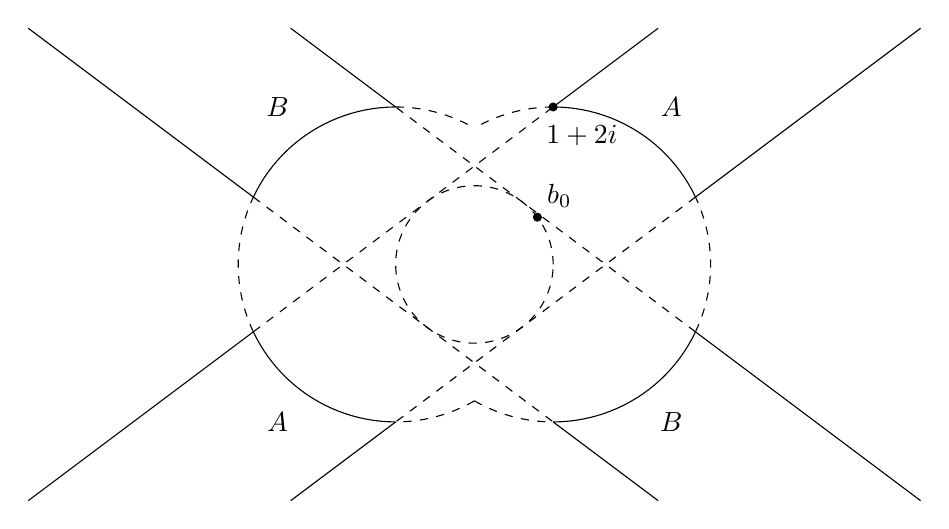
\begin{tikzpicture}
				\draw[black, dashed, domain = -120:-90] plot({1 + 2*cos(\x)}, {2*sin(\x)});
				\draw[black, domain = -90:{-atan((-4 + 6*sqrt(6))/(3 + 8*sqrt(6)))}] plot({1 + 2*cos(\x)}, {2*sin(\x)});
				\draw[black, dashed, domain = {-atan((-4 + 6*sqrt(6))/(3 + 8*sqrt(6)))}:{atan((-4 + 6*sqrt(6))/(3 + 8*sqrt(6)))}] plot({1 + 2*cos(\x)}, {2*sin(\x)});
				\draw[black, domain = {atan((-4 + 6*sqrt(6))/(3 + 8*sqrt(6)))}:90] plot({1 + 2*cos(\x)}, {2*sin(\x)});
				\draw[black, dashed, domain = 90:120] plot({1 + 2*cos(\x)}, {2*sin(\x)});
				
				\draw[black, dashed, domain = -120:-90] plot({-1 - 2*cos(\x)}, {2*sin(\x)});
				\draw[black, domain = -90:{-atan((-4 + 6*sqrt(6))/(3 + 8*sqrt(6)))}] plot({-1 - 2*cos(\x)}, {2*sin(\x)});
				\draw[black, dashed, domain = {-atan((-4 + 6*sqrt(6))/(3 + 8*sqrt(6)))}:{atan((-4 + 6*sqrt(6))/(3 + 8*sqrt(6)))}] plot({-1 - 2*cos(\x)}, {2*sin(\x)});
				\draw[black, domain = {atan((-4 + 6*sqrt(6))/(3 + 8*sqrt(6)))}:90] plot({-1 - 2*cos(\x)}, {2*sin(\x)});
				\draw[black, dashed, domain = 90:120] plot({-1 - 2*cos(\x)}, {2*sin(\x)});
				
				\draw[dashed] (0,0) circle[radius = 1];
				\filldraw (1, 2) circle[radius = 0.05] node[below right, yshift=-3, xshift = -6] {$1+2i$};
				\filldraw ({4/5}, {3/5}) circle[radius = 0.05] node[above right] {$b_0$};
				\draw ({-17/3}, -3) -- ({-(31 + 16*sqrt(6))/25}, {-(-8 + 12*sqrt(6))/25});
				\draw[dashed] ({-(31 + 16*sqrt(6))/25}, {-(-8 + 12*sqrt(6))/25}) -- (1,2);
				\draw (1,2) -- ({7/3},3);
				
				\draw ({-17/3}, 3) -- ({-(31 + 16*sqrt(6))/25}, {(-8 + 12*sqrt(6))/25});
				\draw[dashed] ({-(31 + 16*sqrt(6))/25}, {(-8 + 12*sqrt(6))/25}) -- (1,-2);
				\draw (1,-2) -- ({7/3},-3);

				\draw ({17/3}, 3) -- ({(31 + 16*sqrt(6))/25}, {(-8 + 12*sqrt(6))/25});
				\draw[dashed] ({(31 + 16*sqrt(6))/25}, {(-8 + 12*sqrt(6))/25}) -- (-1,-2);
				\draw (-1, -2) -- ({-7/3},-3);
				
				\draw ({17/3}, -3) -- ({(31 + 16*sqrt(6))/25}, {-(-8 + 12*sqrt(6))/25});
				\draw[dashed] ({(31 + 16*sqrt(6))/25}, {-(-8 + 12*sqrt(6))/25}) -- (-1,2);
				\draw (-1, 2) -- ({-7/3},3);
				
				\node at (2.5, 2) {$A$};
				\node at (-2.5, -2) {$A$};
				\node at (2.5, -2) {$B$};
				\node at (-2.5, 2) {$B$};
			\end{tikzpicture}
			\caption{The sets $A$ and $B$ from~\eqref{eqAandB}.}
			\label{figAandBaredisjoint}
		\end{figure} 
		Finally, for the third point $z_3 \in E$ we just use the estimate $|z_3| \ge \sqrt{3}$, since $z_3 \notin \Omega$. Therefore, the angular measure of the set $C_{z_1} \cup C_{z_2} \cup C_{z_3}$ can be estimated from above by $\alpha = 4\arcsin(1/\sqrt{3}) + 8\arcsin(1/\sqrt{5})$. Since $\alpha < 2\pi$, we can conclude that there exists $b \in \TT$ such that $b \notin C_{z_1} \cup C_{z_2} \cup C_{z_3}$. This $b$ satisfies $|\mathrm{Im}(z/b)| > 1$ for all $z \in E$.
	\end{proof}

\end{document}
